\documentclass{beamer}
\usetheme{Boadilla}

\addtobeamertemplate{block begin}{\setlength\abovedisplayskip{0pt}}


\usepackage[utf8]{inputenc}
\usepackage[T1]{fontenc}
\usepackage[francais]{babel}
\usepackage{amsmath}
\usepackage{amsfonts}
\usepackage{graphicx}
\usepackage{url}
\usepackage{amsthm}
\usepackage{float}
%\usepackage{mathpazo}

%\usepackage{newpx}
\geometry{hmargin=1.2cm,vmargin=0.3cm}

\DeclareMathOperator*{\argmax}{\arg\!\max}
\newtheorem*{Prob}{Problème}
%\newtheorem*{lemma}{Lemme}
\newtheorem*{hypo}{Hypothèse}
\newtheorem*{defi}{Définition}

\title{Soutenance de stage de L3}
\subtitle{Cryptanalyse linéaire expérimentale de DES}
\author{Lucas Pesenti\thanks{Sous la direction de François-Xavier Standaert dans l'équipe UCL Crypto de Louvain-la-Neuve (Belgique).}}
\date{juin -- juillet 2017}

\begin{document}

\begin{frame}
	\maketitle
\end{frame}

\begin{frame}
	\tableofcontents
\end{frame}

\section{Vue d'ensemble de l'attaque}
\begin{frame}
	\tableofcontents[currentsection]
\end{frame}

\subsection{Présentation de DES}
\begin{frame}{Présentation de DES}
	\begin{itemize}
		\item Entrée sur 64 bits.
		\item Clé sur 56 bits.
	\end{itemize}

	\begin{figure}
		\centering
		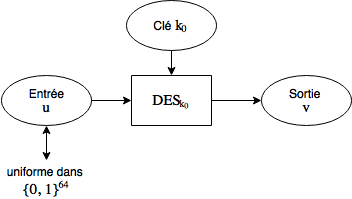
\includegraphics[scale=0.8]{descheme}
	\end{figure}
\end{frame}

\begin{frame}{Présentation de DES (suite)}
	\begin{columns}
	\begin{column}{0.3\textwidth}
	\begin{figure}
		\centering
		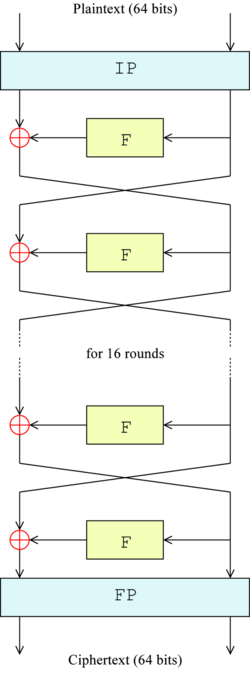
\includegraphics[scale=0.32]{DESwiki}
		\label{deswiki}
	\end{figure}
	\end{column}
	\begin{column}{0.7\textwidth}
	\begin{figure}
		\centering

		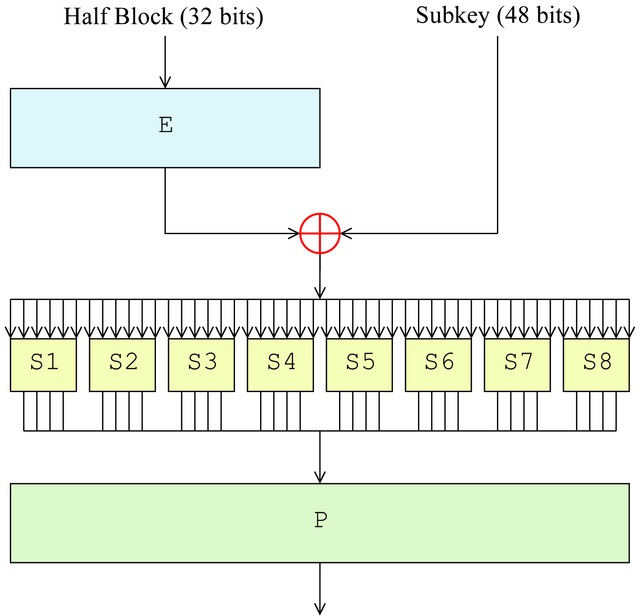
\includegraphics[scale=0.3]{Ffunc}
	\end{figure}
	\end{column}
	\end{columns}
\end{frame}

\subsection{Fonctionnement général de l'attaque}
\begin{frame}{Fonctionnement général de l'algorithme 2 de Matsui}
	\begin{itemize}
		\item $N$ couples clair/chiffré.
		\item Approximations linéaires biaisées entre l'entrée et la sortie.
		\item Déchiffrement partiel.
		\item \textbf{Rang} de la clé : position dans le parcours exhaustif final.
		\item \textbf{Avantage} $a$ si le rang est inférieur à $2^{56-a}$.
	\end{itemize}

	\vspace*{-1cm}
	\begin{columns}
		\begin{column}{0.5\textwidth}
	\begin{figure}
		\centering
		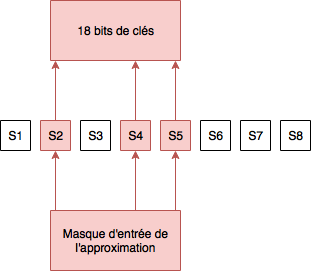
\includegraphics[scale=0.5]{partiel}
	\end{figure}
		\end{column}
		\begin{column}{0.45\textwidth}
			Phase de cryptanalyse linéaire : associer à chacune des $2^{18}$ classes de clés un score.
		\end{column}
	\end{columns}

\end{frame}

\begin{frame}{Déchiffrement partiel}
Nombre de bits de clé de dépendance :
\begin{figure}[H]
\[
\begin{array}{|c|c|c|c|c|c|c|c|c|}
	\hline
	\text{Identifiant de la S-box $j$} & 1 & 2 & 3 & 4 & 5 & 6 & 7 & 8\\
	\hline
	\text{Niveau $i=1$} & 6 & 6 & 6 & 6 & 6 & 6 & 6 & 6\\
	\text{Niveau $i=2$} & 38 & 40 & 39 & 36 & 37 & 36 & 38 & 39\\
	\text{Niveau $i=3$} & 53 & 55 & 52 & 56 & 54 & 55 & 54 & 55\\
	\text{Niveau $i=4$} & 56 & 56 & 56 & 56 & 56 & 56 & 56 & 56\\
	\hline
\end{array}
\]
\end{figure}

1 round déchiffré partiellement en entrée, 1 en sortie.
\end{frame}

\begin{frame}{Fonctionnement général de l'attaque}
	\begin{itemize}
	\item Attaque linéaire multidimensionnelle.
	\item Combinaison de plusieurs attaques indépendantes.
	\end{itemize}

	\begin{figure}
		\centering
		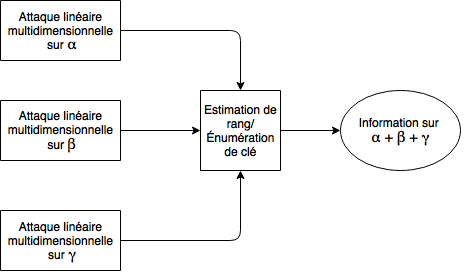
\includegraphics[scale=0.6]{multi}

		$\alpha,\beta,\gamma$ : masques de la clé
	\end{figure}
\end{frame}

\section{Génération des approximations linéaires}
\begin{frame}
	\tableofcontents[currentsection]
\end{frame}

\subsection{Généralités}
\begin{frame}{Schéma de la génération des approximations linéaires}
	\begin{figure}
		\centering
		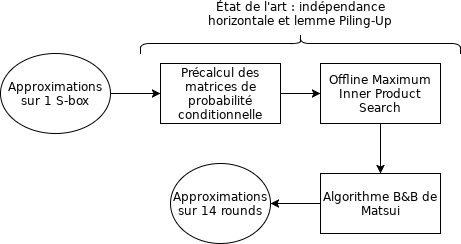
\includegraphics[scale=0.6]{genscheme}
	\end{figure}
\end{frame}

\begin{frame}{Définitions}
	\begin{defi}[approximation linéaire]
	\begin{itemize}
		\item Approximation linéaire $\alpha \cdot u + \beta \cdot v=\gamma \cdot k_0$ de biais :
			
	$$\epsilon=\left|P(\alpha \cdot u + \beta \cdot v=\gamma \cdot k_0)-\frac{1}{2}\right|$$

	\item Système de $m$ approximations linéaires $Au+Bv=\Gamma k_0$ de capacité :

	$$C=\sum_{\eta=0}^{2^m-1}\left(P(Au+Bv=\eta)-\frac{1}{2^m}\right)^2$$
	\end{itemize}
	\end{defi}
\end{frame}

\subsection{Combinaison d'approximations}
\begin{frame}{Combinaison d'approximations}
\begin{lemma}[Piling-Up]
	Si $X_1, \ldots X_n$ sont des variables aléatoires indépendantes à valeurs dans $\{0,1\}$, alors :
$$P(X_1 + \ldots + X_n=0)=\frac{1}{2}+2^{n-1}\prod_{i=1}^n \left(P(X_i=0)-\frac{1}{2}\right)$$
\end{lemma}

	\begin{figure}
		\centering
		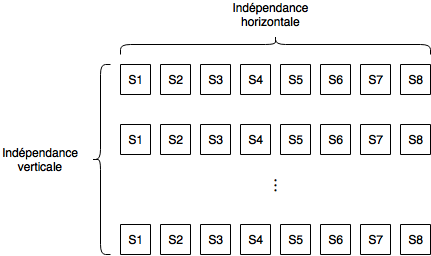
\includegraphics[scale=0.5]{indep}
	\end{figure}
\end{frame}

\begin{frame}{Hypothèse d'indépendance horizontale}
\begin{figure}[H]
	\centering
	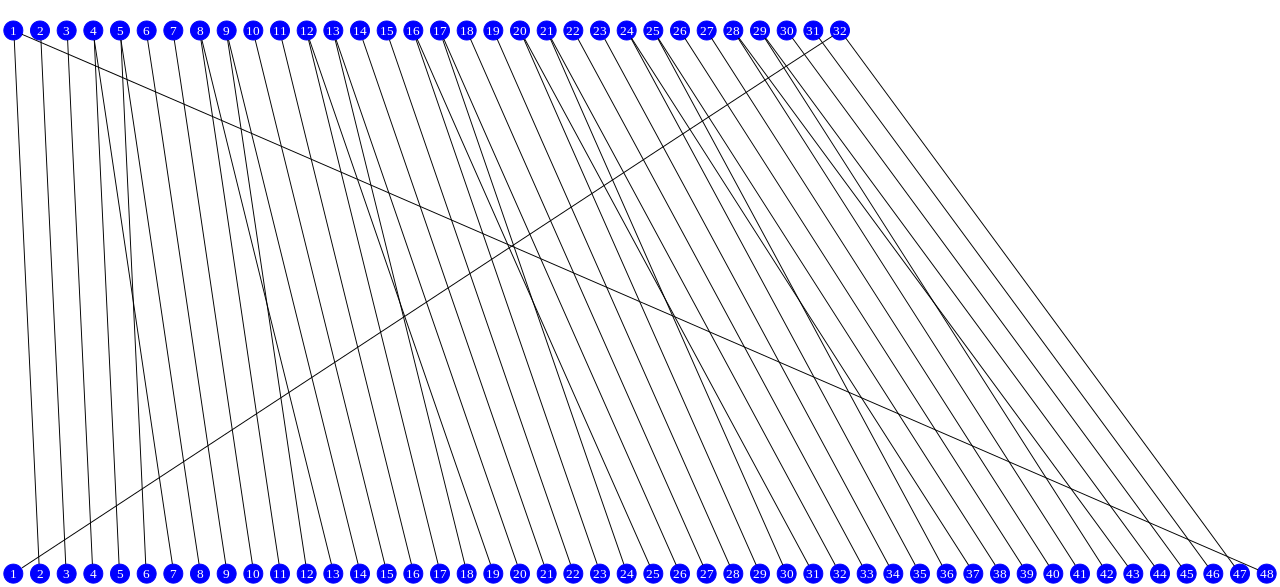
\includegraphics[scale=0.25]{exp}

	Schéma de la fonction d'expansion (Wikipedia)
\end{figure}
\end{frame}

\subsection{Génération des approximations sur 1 round}
\begin{frame}{Génération des approximations sur 1 round}
	\begin{Prob}[OFF-MIPS]
	Entrée : $(l_i)_{1\le i\le n}$ et $(r_j)_{1\le j\le n}$ vecteurs de $\mathbf{R}^d$.

	Sortie :
		$$\underset{1\le j\le n}{\underset{1\le i\le n}{\argmax}}\langle l_i,r_j\rangle$$
	\end{Prob}

	\begin{itemize}
		\item Réduction à OFF-MIPS : précalcul de matrices $4\times 4$ des biais sur 1 S-box.
		\item Résolution de OFF-MIPS : algorithme probabiliste.
	\end{itemize}
\end{frame}

\subsection{Résultats}
\begin{frame}{Résultats}
	Algorithme B\&B de Matsui :
	\begin{itemize}
		\item Plus court chemin dans un DAG, arêtes de poids positif, $2^{100}$ n\oe{}uds, $2^{132}$ arêtes.
		\item Matsui : élagage intelligent.
		\item En pratique : plus efficace que la génération sur 1 round.
	\end{itemize}
	
	Résultats :
	\begin{itemize}
		\item Simulation de 6h sur un bon serveur.
		\item Pas de changement de biais pour les approximations principales.
		\item Multithreading envisagé.
		\item $\sim 1400$ masques de clé distincts.
	\end{itemize}
\end{frame}

\section{Phase d'attaque}
\begin{frame}
	\tableofcontents[currentsection]
\end{frame}

\subsection{Cryptanalyse multilinéaire (modèle d'Hermelin)}
\begin{frame}{Cryptanalyse multilinéaire (modèle d'Hermelin)}
$$Au^{k_0}+Bv^{k_0}=\Gamma k_0$$

\begin{hypo}[de la mauvaise clé]
	Si $k\neq k_0$ et si $u^{k}$ et $v^{k}$ sont déchiffrés partiellement avec la clé $k$, alors
$Au^{k}+Bv^{k}$ suit une distribution uniforme.
\end{hypo}

Test statistique :
	\begin{itemize}
		\item si $k=k_0$ : distribution jointe (biaisée).
		\item si $k\neq k_0$ : distribution uniforme.
	\end{itemize}

\begin{defi}[distribution empirique]
$$P(k,\eta)=\text{Card}\{i\in\{1,\ldots,N\} | Ax_i^k+By_i^k=\eta\}$$
\end{defi}

Test du $\chi^2$ : $S(k)=\sum_{\eta=0}^{2^m-1} \left(\frac{P(k,\eta)}{N}-\frac{1}{2^m}\right)^2$
\end{frame}

\begin{frame}{Des scores aux probabilités}
Modèle bayésien :

	\begin{itemize}
		\item $D=\chi^2_{2^m-1}(NC)$ : distribution limite quand $N\to\infty$ de $2^mNS(k)$ si $k=k_0$.
		\item $D'=\chi^2_{2^m-1}(0)$ : idem si $k\neq k_0$.
	\end{itemize}


\begin{align*}
	P(k=k_0|S=s)=\text{cte}\times \frac{f_D(S(k))}{f_{D'}(S(k))}
\end{align*}


\end{frame}

\subsection{Optimisation temporelle du déchiffrement partiel}
\begin{frame}{Optimisation temporelle du déchiffrement partiel}

Rappel des notations :
	\begin{itemize}
		\item $N$ : nombre de couples clair/chiffré.
		\item $m$ : nombre d'approximations.
		\item $t$ : cardinal du masque de clé.
	\end{itemize}

Complexités temporelles :
\begin{itemize}
	\item Complexité naïve : $O(Nm2^t)$.
	\item Optimisation de Matsui avec précalcul : $O(N+m2^{2t+m})$.
	\item (non implémenté entièrement) Optimisation de Nguyen avec transformée de Fourier/Walsh-Hadamard : $O(N+(t+m)2^{t+m})$.
\end{itemize}
\end{frame}

\subsection{Estimation de rang}
\begin{frame}{Estimation de rang}
	\begin{itemize}
		\item Outils développés dans mon équipe d'accueil.
		\item Combine des listes de probabilité pour obtenir une estimation du rang de la clé
		si on les parcourt par probabilité décroissante.
		\item Contrainte : morceaux de clé disjoints.
	\end{itemize}
\end{frame}

\begin{frame}{Combinaison d'attaques multilinéaires}

\begin{itemize}
	\item Avantage fournie par chaque liste connu (Hermelin).
	\item Combinaison de deux listes de masques de clé disjoints : avantage sommé.
	\item Compression d'une liste en un masque plus petit : avantage réduit du nombre de bits compressés.
\end{itemize}

	\vspace{-0.2cm}
\begin{Prob}
Maximiser l'avantage d'une liste pouvant être obtenue par combinaisons et compressions des listes de départ.
\end{Prob}
	\vspace{-0.5cm}

	\begin{columns}
		\begin{column}{0.5\textwidth}
\begin{figure}
	\centering
	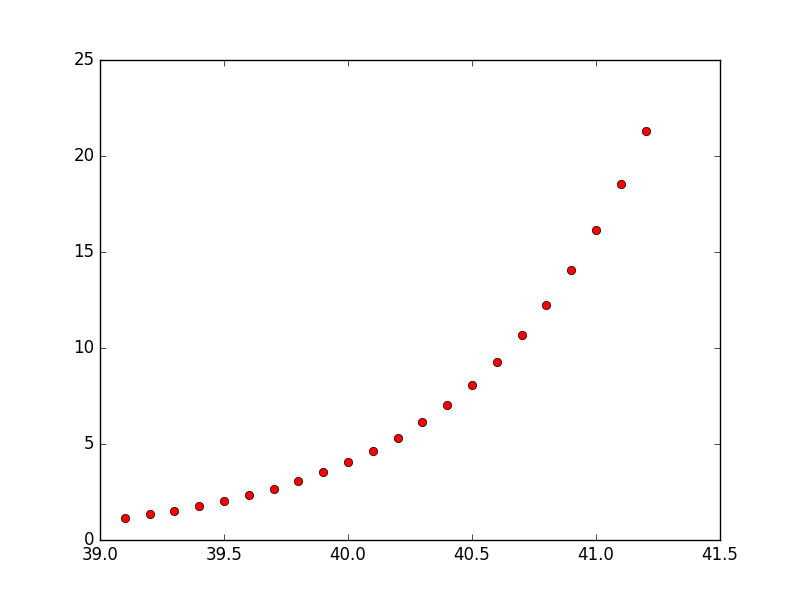
\includegraphics[scale=0.25]{fig1}
%	\caption{Meilleur avantage théorique en fonction du logarithme de la complexité en donnée pour le DES sur 14 rounds. Tous les
%	points correspondent en fait à la combinaison des deux listes d'approximations de Matsui.}
%	\label{reftheo}
\end{figure}
		\end{column}
		\begin{column}{0.45\textwidth}
Résultats avec une file à priorité sur 14 rounds : meilleurs biais théoriques obtenus avec les approximations de Matsui.
		\end{column}
	\end{columns}

\end{frame}

\subsection{Résultats de l'attaque}
\begin{frame}{Résultats de l'attaque sur 8 rounds}

\begin{figure}
	\[
		\begin{array}{|c|c|}
			\hline
			\text{Biais 1} & \text{Biais 2}\\
			\hline
			1.4648 \times 2^{-11} & 1.1250\times 2^{-12}\\
			\hline
			1.4648 \times 2^{-12} & 1.1250\times 2^{-13} \\
			\hline
			1.6875 \times 2^{-15} & 1.1250\times 2^{-13}\\
			\hline
		\end{array}
	\]
	\caption{Biais des approximations choisies}
\end{figure}
	\vspace{-1cm}
\begin{figure}
\[
	\begin{array}{|c|c|c|c|c|c|c|c|}
		\hline
		N & 2^{20} & 2^{22} & 2^{23} & 2^{24} & 2^{25} & 2^{25.5} & 2^{26}\\
		\hline
		R_{\text{min}} & 2^{54.205} & 2^{54.652} & 2^{40.340} & 2^{34} & 2^{41.175} & 2^{36} & 2^{32}\\
		\hline
		R_{\text{round}} & 2^{54.211} & 2^{54.658} & 2^{40.384} & 2^{34.322} & 2^{41.224} & 2^{36.170} & 2^{33}\\
		\hline
		R_{\text{max}} & 2^{54.211} & 2^{54.658} & 2^{40.384} & 2^{34.322} & 2^{41.224} & 2^{36.170} & 2^{33}\\
		\hline
		a_{\text{round}} & 1.789 & 1.342 & 15.616 & 21.618 & 14.776 & 19.830 & 23\\
		\hline
	\end{array}
\]
	\caption{Résultats des simulations}
\end{figure}

\end{frame}


\begin{frame}{Conclusion}
	\begin{itemize}
		\item Attaque complète du DES avec des outils nouveaux.
		\item Nécessité d'un outil pour faire de l'estimation de rang avec dépendance.
		\item Résultats difficiles à interpréter.
		\item Introduction à la cryptanalyse et à la recherche.
	\end{itemize}
\end{frame}

\begin{frame}{Bibliographie}
\nocite{*}
\bibliography{biblio}
\bibliographystyle{alpha}
\end{frame}
\end{document}
